\section{Preparation for the Muscles and the System}\label{section_preparation}
\scps respond to a function of temperature. In order to precisely control the complicated system, an electrical microprocessor was used. Therefore, the methods for electrically operating \scps and investigating their characteristics are discussed in this section. 

\subsection{Fabrication of the SCP Artificial Muscles}
The \scps used in this paper were made by twisting silver-painted nylon thread (Conductive Sewing Thread Size 92, Shieldex), which was found to be best in terms of strain and force production \cite{haines}. First, the conductive thread was piled up four times to make its length be \SI{50}{\centi\meter}. Each side of thread was connected to washers. Then, a wire was hung to one of the washer and a motor to the other. (Fig.\ref{silverSCP_2})
As illustrated in Fig.\ref{silverSCP_illust}, the motor was rotated until the thread creates a coil \cite{fab_coil}. After making same one again, two coils were overlapped to each other, making stable form. 
Lastly, they were heated up under an electric current.\footnote{\SI{2.5}{\ampere} was applied and stopped when smoke occurred. While repeating heating and cooling about ten times, the length at ambient temperature got longer and reached at a constant length.} By this method, we made a \scp which is \SI{10}{\centi\meter} - \SI{11}{\centi\meter} in length and \SI{2.5}{\ohm} in electric resistance at ambient temperature with no external force.

\begin{figure}
	\centering
	\begin{subfigure}{.15\linewidth}
		\centering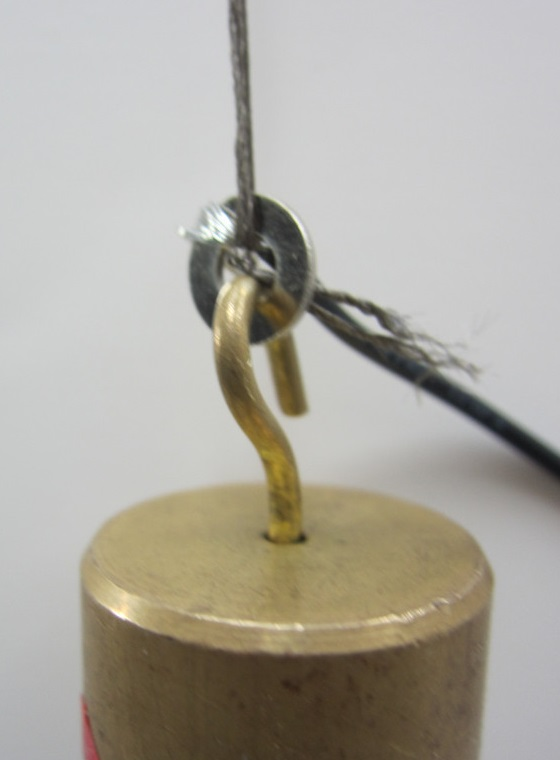
\includegraphics[width=\textwidth]{small_silverSCP_3_v2.jpg}
		\caption{\label{silverSCP_2}}
	\end{subfigure}
	~
	\begin{subfigure}{.45\linewidth}
		\centering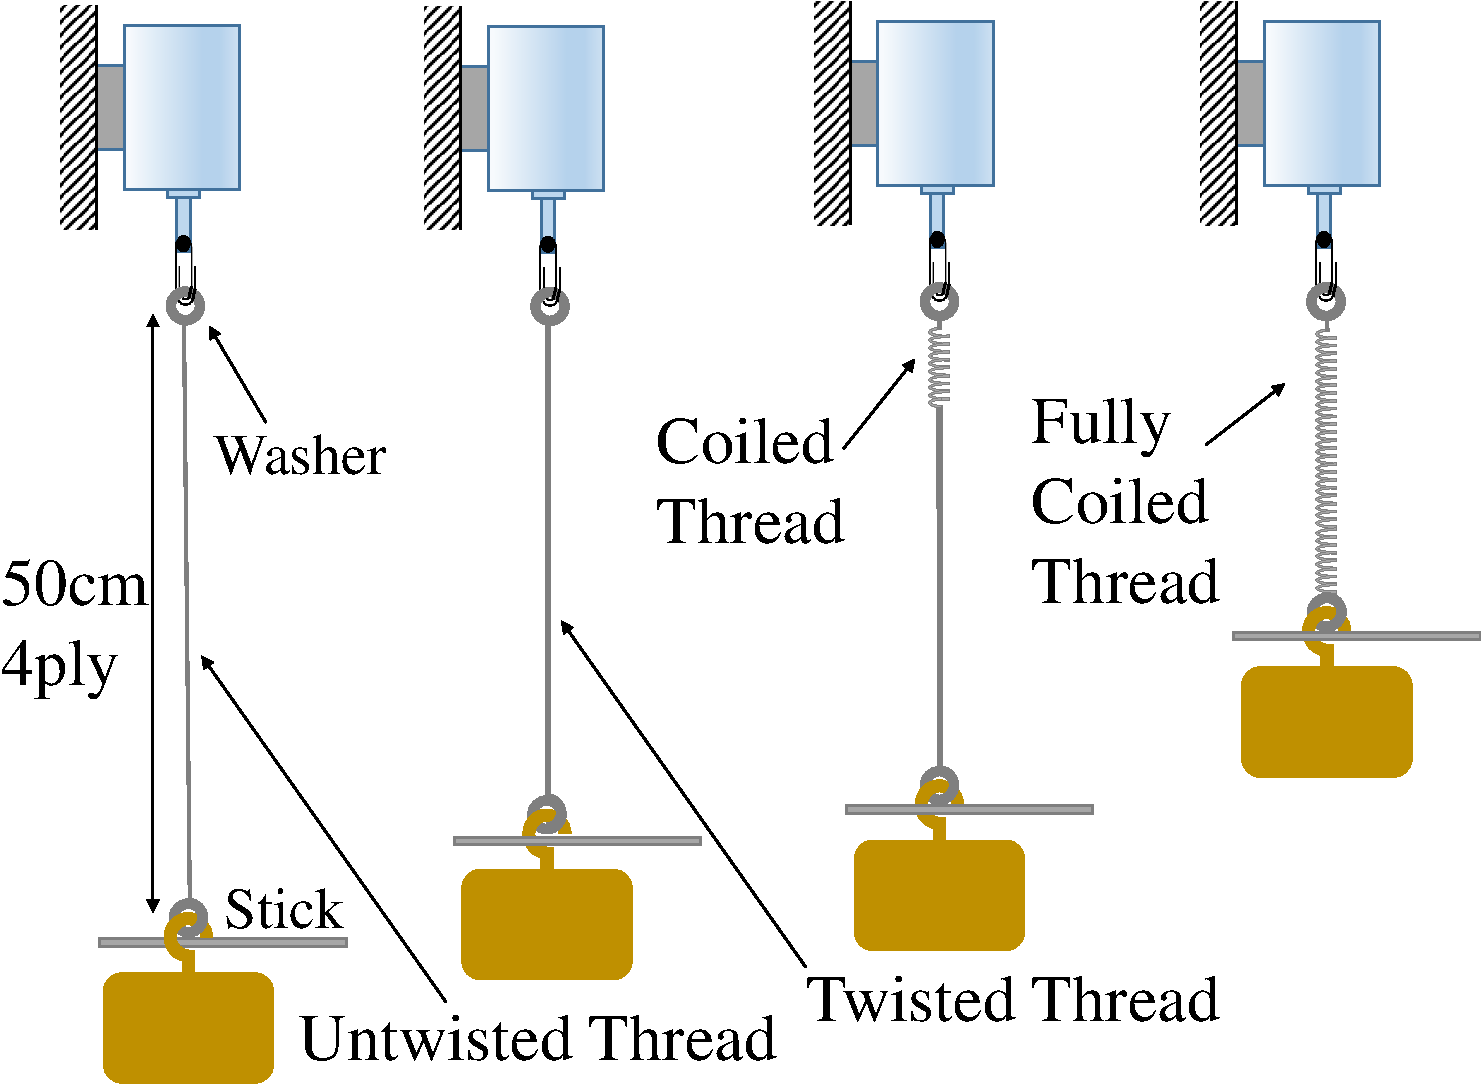
\includegraphics[width=\textwidth]{Fab_illust_v2_crop.pdf}
		\caption{\label{silverSCP_illust}}
	\end{subfigure}
	~
%	\begin{subfigure}{.12\linewidth}
%		\centering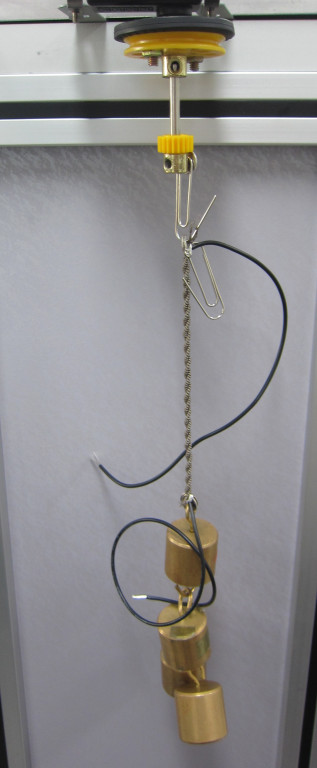
\includegraphics[width=\textwidth]{small_silverSCP_6.jpg}
%		\caption{\label{silverSCP_6}}
%	\end{subfigure}
%	~
	\begin{subfigure}{.15\linewidth}
		\centering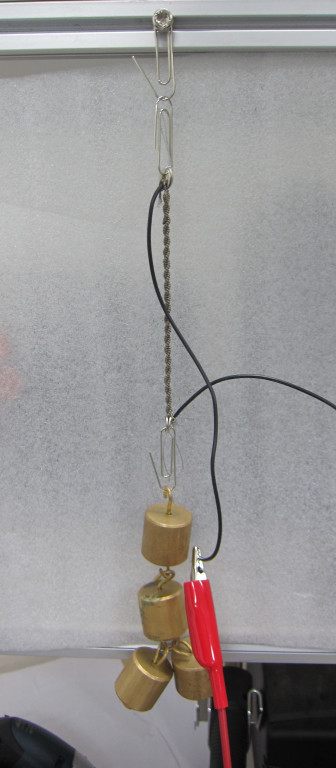
\includegraphics[width=\textwidth]{small_silverSCP_7.jpg}
		\caption{\label{silverSCP_annealing}}
	\end{subfigure}
	\caption[Process of making \scps with silver-painted nylon thread]{\subref{silverSCP_2} 4-ply, \SI{50}{\centi\meter} thread bundle's each side was hung on washers. The upper end was hung on motor, and the lower end was hung on \SI{400}{\gram} weight with a wire inserted in between washer and thread. \subref{silverSCP_illust} In order to twist a thread until it creates a coil, the bottom was fixed with a stick. Then, two super coiled polymers were made. Their upper parts were hung on one clip and their lower parts were hung on \SI{400}{\gram} weight. Coiled thread's thickness was exaggerated. \subref{silverSCP_annealing} By these processes, the \scpnospace, which has wire on its each side, was made. Finally, they were annealed until their length at ambient temperature didn't get longer.}
	\label{silverSCP_makingof}
\end{figure}

\subsection{Electrical Control of the SCP Artificial Muscles}\label{section_electrical_control}
As discussed in the previous section, the \scp was made with conductive thread in order to electrically control heat speed. Electrical resistance of the \scp was $R=\SI{2.5}{\ohm}$, so the power $P$ was supplied by applying voltage $V=\sqrt{PR}$. The voltage was controlled by MOSFET and PWM generation of Arduino Uno.

In order to implement faster cooling speed of the \scp, a compressed air tank and a solenoid valve were used. The air tank forced air(temperature : equals to  $T_{ambient}$) to flow around the \scp, so we can significantly increase the thermal conductivity of the muscle. Meanwhile, the amount of air flow couldn't be analog controlled. Therefore, by stopping and resuming the flow of air with an appropriate period and ratio, we could control the thermal conductivity of the muscle. This will be discussed at section \ref{section_dynamic} in more details.

\subsection{Physical Measurements of the SCP Artificial Muscles}
Physical properties of the \scps, such as temperature, length, and tension, were measured with various sensors.
\footnote{For the detailed information of sensors, see Table \ref{used_materials}.}
SMD type temperature sensor was used to measure the temperature of the \scps without effecting the specific heat of the \scpnospace.

Also, a slide potentiometer was utilized to measure the linear displacement of the \scpsnospace. However, since it had significant amount of friction, it was only used for the experiments about \scpnospace's characteristics. On the other hand, rotary sensor, which has low frictional torque, was employed to make an \antanospace. 

To measure the tension of the \scpsnospace, a load cell and an amplifier were used.
The load cell played a role in connecting the \scps and the skeleton of the \antanospace.
% As seen as Fig.\ref{anta_loadcell}, load cell played a role of connecting \scp and skeleton of \anta.

\subsection{An \ANTA}
\scps can be easily heated by applying electric current. However, cooling demands more sophisticated procedure. Also, muscles can produce force only when contracting, not for relaxing. This means that \scps can't be directly applied to robots which have to produce force in various positions.
Therefore, we used a principle of antagonism, which is known to be energy-optimal for various tasks \cite{antagonism}.

An \anta was made with two \scpsnospace, which can produce stronger force in two positions within a short time than a single \scpnospace.
First, we made a skeleton of the \anta with 3D printer. (Fig.\ref{3d_assemblies}) Then, non-elongating wire was used to connect stand, muscle, and ball bearing with a rotary sensor inside. A cooling device was also attached to the two \scpsnospace. Lastly, sensors of \anta were connected to Arduino Uno with PCB. (Fig.\ref{anta_overall})

\begin{figure}[t]
	%add desired spacing between images, e. g. ~, \quad, \qquad, \hfill etc. 
	%(or a blank line to force the subfigure onto a new line)
	\centering
	\begin{subfigure}[t]{0.5\textwidth}
		\centering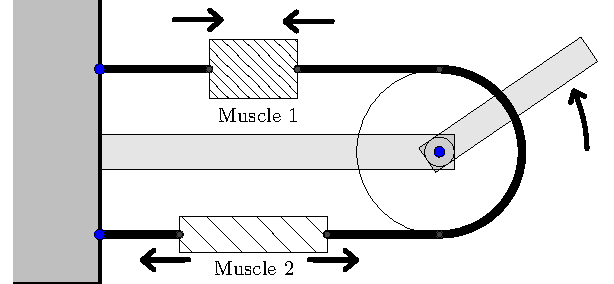
\includegraphics[width=\textwidth]{AntaSchematic_v3.pdf}
		\caption{\label{anta_sch}}
	\end{subfigure}
	~			
	\begin{subfigure}[t]{0.3\textwidth}
		\centering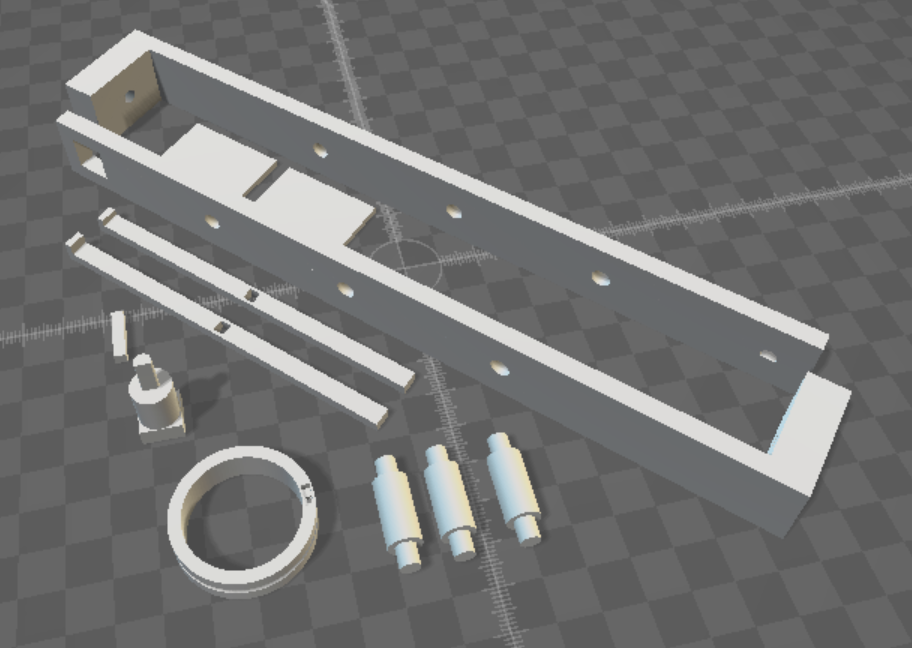
\includegraphics[width=\textwidth]{Anta_3d_assemblies_v2.png}
		\caption{\label{3d_assemblies}}
	\end{subfigure}
	
	\begin{subfigure}[t]{0.81\textwidth}
		\centering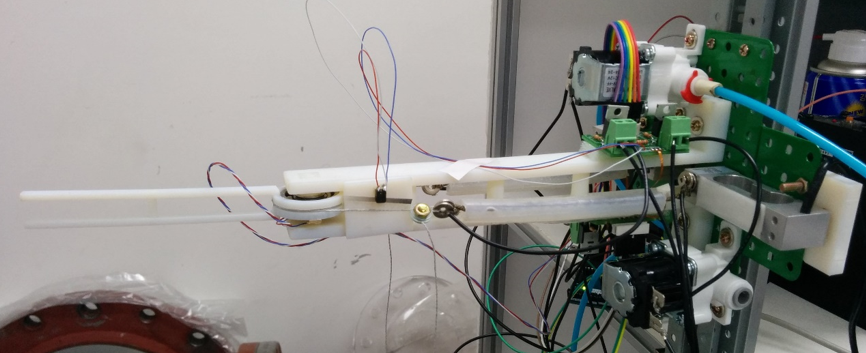
\includegraphics[width=\textwidth]{Anta_overall_v2.png}
		\caption{\label{anta_overall}}
	\end{subfigure}
	
	\caption[An \Anta]{\subref{anta_sch} By contracting two \scpnospace s complementarily, we could get the same effect as cooling one muscle by heating another. \subref{3d_assemblies} The skeleton of the \anta was designed with the software(3D Builder, Microsoft) and 3d-printed. \subref{anta_overall} An overall image of the \anta was as above.}
	\label{anta_design}
\end{figure}
